\epigraph{\textit{The most damaging phrase in the English language is "we have always done it this way".}}{-- \textup{Grace Hopper}}

We have examined two distinct Scala and Apache Spark-based solutions up to this point. Both were, as we have mentioned, far from ideal. We have to start from scratch if we want to find a more sophisticated solution.

\section{Technology stack}

\begin{figure}[ht]
    \newsavebox\mybox
    \savebox{\mybox}{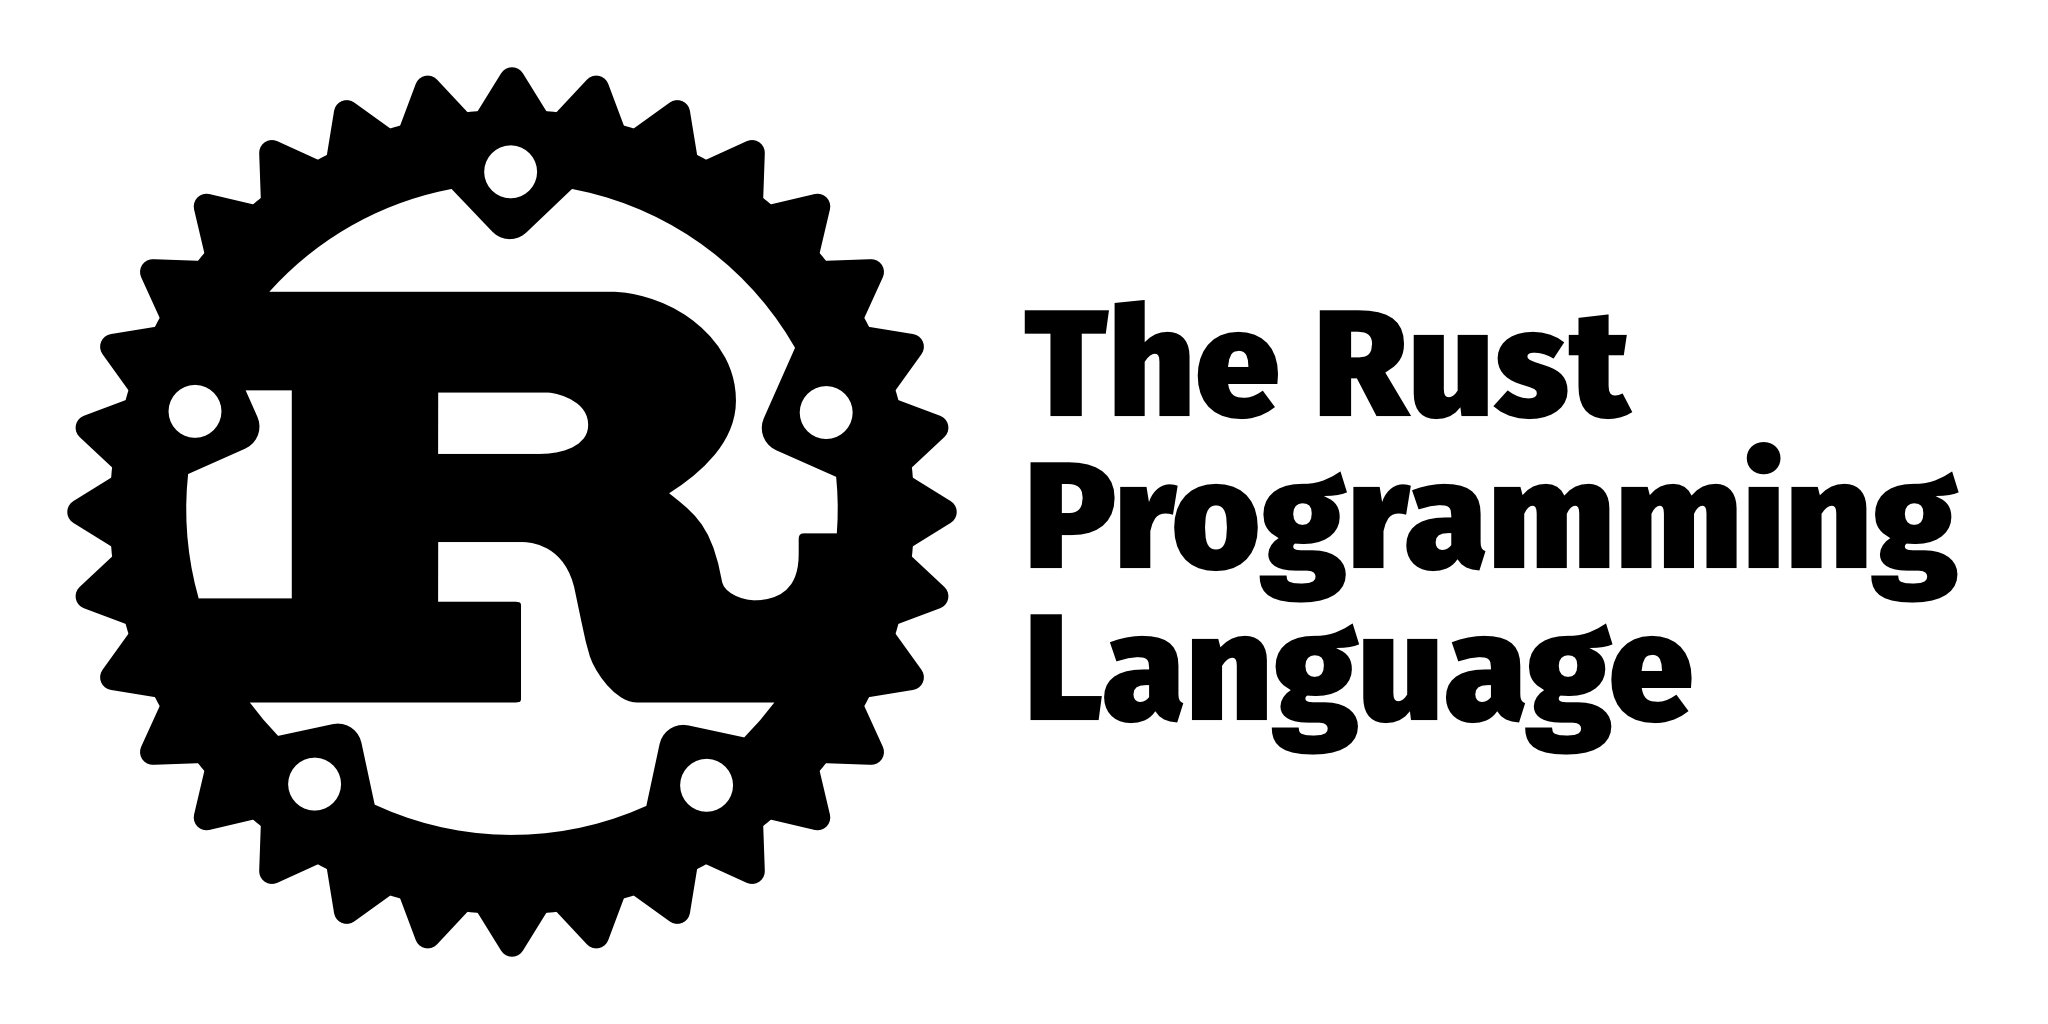
\includegraphics[width=.4\linewidth]{img/9-1_rust.jpg}}

    \begin{subfigure}{.45\textwidth}
        \centering
        \usebox{\mybox}
        \caption{Rust programming language}
    \end{subfigure}%
    \hspace*{0.5em}
    \begin{subfigure}{.45\textwidth}
        \centering
        \vbox to \ht\mybox{%
            \vfill
            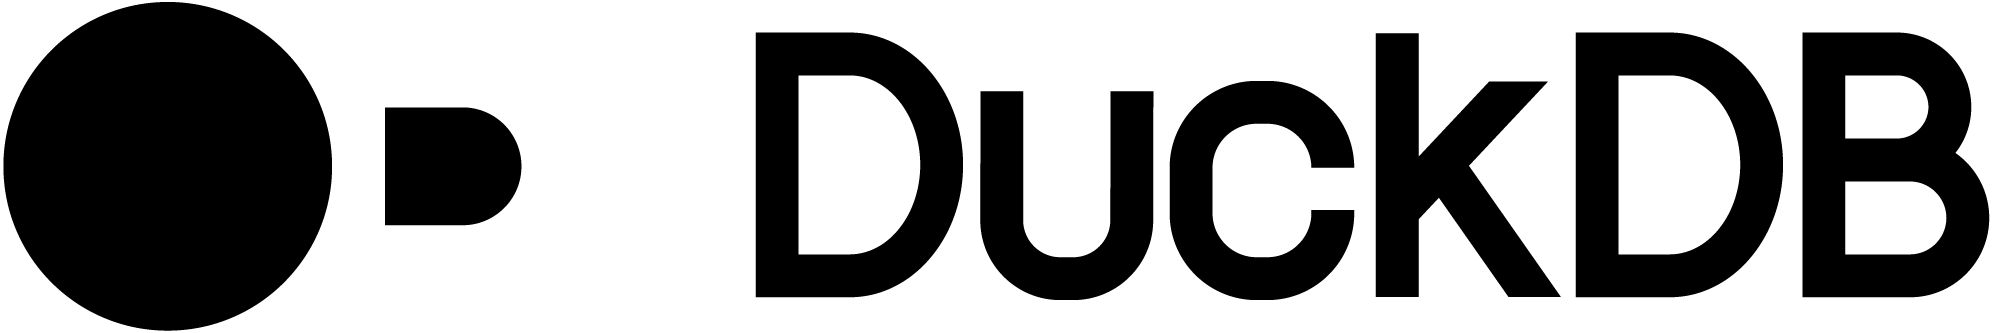
\includegraphics[width=.8\linewidth]{img/9-2_duckdb.png}
            \vfill
        }
        \caption{DuckDB}
    \end{subfigure}%
    \caption{Stack of the different technologies we are using for the third solution}
\end{figure}

\subsection{Rust}

Rust is a multi-purpose, high-level, and general-purpose programming language. Its primary focus is on performance, memory safety, and concurrency. In this perspective, Rust might be considered a modern language; as of March 18th, 2023, the most recent stable release is version 1.68. For achieving memory safety and concurrency, both at the same time, Rust prevents data races through a \textit{borrow checker} that tracks the object and allows each memory position to have only one owner at a time. Rust is popular for systems programming, and was included by the Linux kernel in December 2022, but it also has some high-level functional constructs like pattern-matching and the neatly implemented \texttt{Enums}.

\begin{code}[Hello World written in Rust]
    \inputminted{rust}{code/listings/9-1_helloWorld.rs}
\end{code}

\subsection{DuckDB}